\chapter{Performance Evaluation}
\label{chapter:evaluations}
In this chapter we first introduce the datasets that we use for evaluating the efficacy of our document representations for the document categorization task. We then explain the details of our experimentation setup and the different document representation techniques that form strong baselines that we compare our model to. In the sections following that we present the results for assigning categories to new documents and also imputing missing categories for documents for which we already have prior category information. 

\section{Datasets}
We perform our experimentation on 5 datasets that contain rich data about documents belonging to multiple categories simultaneously. One of the 5 datasets we use is the famous Reuters-21578 collection, which is considered the benchmark for text classification evaluation. Along with the being richly multi-label and large-sized, Reuters-21578 has been used for many years for evaluation which gives us the opportunity to compare our accuracy with the previous state-of-the-art results. The other 4 datasets that we evaluate on are, exclusive subsets of documents, extracted from Wikipedia.


\subsection{Reuters-21578}
Reuters-21578 collection consists of documents published on the Reuters newswire in 1987. As the name suggests it has a total of 21758 documents assigned categories from a set of 135 categories. Though most of the documents in the collection are multi-labeled, many documents are assigned only a single category. The Reuters-21578 dataset has over the years become a standard dataset for evaluating many information retrieval algorithms due to the the multi-label nature of the collection and the large number of categories present in the collection that are overlapping and non-exhaustive. Relationships between the categories also makes it an interesting dataset to evaluate on, as the algorithms that capture the correlations between the categories are bound to perform better. Even though the dataset contains large number of documents and categories, it is very sparse making the learning difficult.

Though there exist many processed versions of the collection, the \emph{ModApte} (Modified Apte) version is the most widely used version of the Reuters-21578 for evaluating multi-label classification algorithms. The \emph{ModApte} version predefines a train/test split by considering all documents published after a specific date for testing purposes and the rest for training. After the split, only categories considered are the ones that have atleast one document in the training and the test set. The number of documents, categories, words and other statistics of the Reuters(\emph{ModApte}) dataset are given in Table~\ref{reuter:data:stat}.

\begin{table}[h!]
%\tabcolsep=0.05cm
%\footnotesize
\begin{center}
\begin{tabular}{l c c c c c} % ccc ccc}
\toprule
& \textbf{$|\setD|$} & \textbf{$|\setC|$} & \textbf{$|\setW|$} & \textbf{Data Points} & \textbf{Sparsity}\\
\midrule
\textbf{Train Set}	& 7,767 & 90 & 39,853 & 9,585 & 0.0137 \\
\textbf{Test Set}	& 3,019 & 90 & 39,853 & 3,745 & 0.0138 \\
\bottomrule         
\end{tabular}
\caption{\label{reuter:data:stat}Statistics of the Reuters-21578 (\emph{ModApte}) Dataset}
\end{center}
\end{table}

\subsection{Wikipedia Datasets}
Wikipedia\footnote{www.wikipedia.org} is a free-access free content Internet encyclopedia that contains articles about virtually anything possible. Along with the humongous amounts of articles, Wikipedia also has a hierarchical cyclic \emph{Wikipedia Category Graph} that is used to label articles with the categories they belong in. 
Though the category graph is completely connected, it has few major top-level categories within which all subsequent categories fall. For eg. some of the top-level categories are \emph{Culture and Arts}, \emph{Geography}, \emph{Health}, \emph{History}, \emph{Mathematics}, \emph{Natural and Physical Sciences}, \emph{Philosophy} etc. Each of the top-level categories are further divided into deep trees of fine-grained categories that are assigned to the articles. 

The categories that are assigned to an article thus ranges from broader categories to much fine-grained that are very difficult to assign via an automated system. For eg. some of the categories assigned to an article on the musician \emph{Jimi Hendrix} are \emph{1942 Births}, \emph{1970 deaths}, \emph{American Rock Guitarists}, \emph{Musicians from Seattle}, \emph{Military Brats}, \emph{Alcohol-related deaths in England}. Automatic categorization of such granularity requires the document representation to capture the different semantic topics in the document with great accuracy.

To test the efficacy of our model on such a diverse, recent and real-life dataset, we extracted documents from 4 top-level categories in Wikipedia, namely \emph{Physics}, \emph{Biology}, \emph{Mathematics} and \emph{Sports}, in the following manner. For each of the top-level category we compiled a list of all its child categories till a 3-level depth. To create the document-category dataset, we considered all the documents and the assigned categories, that belonged to the compiled category list. The number of documents, categories, words and other statistics of the extracted datasets are given in Table~\ref{wiki:data:stat}.

\begin{table}[h!]
%\tabcolsep=0.05cm
%\footnotesize
\begin{center}
\begin{tabular}{l c c c c c} % ccc ccc}
\toprule
& \textbf{$|\setD|$} & \textbf{$|\setC|$} & \textbf{$|\setW|$} & \textbf{Data Points} & \textbf{Sparsity}\\
\midrule
\textbf{Physics}		& 4,229 & 2,999 & 81,614 & 14,070 & 0.0010 \\
\textbf{Biology}		& 1,604 & 2,051 & 63,767 & 5,908 & 0.0018 \\
\textbf{Sports}			& 1,529 & 2,829 & 59,058 & 3,745 & 0.0008 \\
\textbf{Mathematics}	& 1,193 & 1,519 & 43,398 & 3,916 & 0.0013 \\
\bottomrule         
\end{tabular}
\caption{\label{wiki:data:stat}Statistics of the Wikipedia Datasets}
\end{center}
\end{table}

\section{Experimental Setup}
\label{sec:exp_setup}
In this section we describe in detail the data preprocessing steps, how we tune the hyper-parameters for both the document representation learning and the categorization algorithm, our evaluation techniques and the baselines we compare to.

\para{Data Preprocessing} : To curate the documents for learning their distributed representations we first split each document at sentence boundaries. We consider different sentences separately because we expect our system to learn syntactic qualities of the language which would not be possible if the sentence boundaries are ignored.
All independent numbers in the documents are converted to `$\backslash num$' and numbers that are a part of a word are left as it is. Eg. \emph{TH1RT3EN}, \emph{Se7en}. 
To remove noise in the documents we only consider those words that occur atleast $5$ times in the corpus.
We preserve the capitalization of the words as, capitalization sometimes encodes a lot of semantic content that we do not wish to lose. Eg. \emph{Apple} in most cases is used to refer to \emph{Apple Inc.} (Company) rather than the fruit, \emph{apple}. Models that distinguish between the two forms should learn better embeddings.

\para{Learning Document Representations} : To learn document representations using our model, we initialize the documents and word embeddings to small random vectors whose elements are drawn uniformly from the range $[-\frac{1}{k}, \frac{1}{k}]$. 
The value of the hyper-parameters of the representation learning model are chosen based on the performance on development data on the end-task of categorization. 
We could also choose the optimum hyper-parameters that minimize the development data perplexity on the document embedding learning task but as found in \citep{mnih2013learning}, lower perplexity does not ensure better representations but could also mean under-training. 
To choose the hyper-parameters we first use the default values as $k = 100$, $c = 2$, $n = 10$, \emph{number of epochs = 50}, $\gamma = 0.0025$, $\beta = 0.1$. 
We found that the learning rate $\gamma$ and the regularization constant $\beta$ give best performance across datasets at their default value. To choose the value of the other parameters, we first tune the embedding dimensions $k$ then the \emph{number of epochs} after which we consider different window sizes ($c$) and finally the number of negative samples $n$ for noise contrastive estimation. The values of the different hyper-parameters depend on the dataset. 
The noise distribution, $P_{n}(w)$ for NCE is chosen to be unigram distribution $U(w)$ raised to the $3/4rd$ power (i.e. $U(w)^{\frac{3}{4}}/Z$) where $Z$ is the normalization factor. Other common choices for noise distribution are uniform distribution and unigram distribution but as found in previous works, $P_{n}(w) \sim U(w)^{\frac{3}{4}}$ works best.

\para{Document Categorization} : For the task of document categorization, we split the document category data into training, development and test data by keeping $10\%$ documents for test purposes and $10\%$ for development. The rest $80\%$ are used for training purposes, i.e. learning category representations. We stop the training based on the convergence reached on the development data. The value of the learning rate $\gamma = 0.01$ and regularization constant $\beta = 0.01$ is chosen based on the performance on development data across different datasets. To make final binary predictions from the estimated probability we need to threshold it, value for which was chosen based on the development data across datasets. It was found that the default logistic threshold of $0.5$ gave the best performance.

\para{Evaluation Criteria} : To evaluate the task of multi-label classification many evaluation criteria such as \emph{Hamming Loss}, \emph{Accuracy} and \emph{F1 score} have been used. We use the \emph{F1} score i.e. the harmonic mean of the precision and recall values to evaluate our model as the F1 score is a much more preferred measure compared to hamming loss or accuracy in the presence of imbalanced label distribution. We compute the F1 score in the micro-averaged fashion by combining prediction values for all the categories together for a particular dataset and then computing the precision and recall values. 
Such averaging ensures equal weightage to all test instances.

\para{Baselines} : To test the efficiency of our document representation learning algorithm, we compare our model's performance to some of the baseline methods that are explained below.
\begin{enumerate}
\item \textbf{Bag-of-Words} : 
The most widely used document representation is the bag-of-words representation with tf-idf weighting. It has been used to produce state-of-the-art results with various learning algorithms. We call this model the \textbf{BOW} model.

\item \textbf{Latent Semantic Indexing} : 
As explained in Sec~\ref{sec:rw_dr}, Latent Semantic Indexing is a popular dimensionality reduction technique that uses the term co-occurrence statistics to capture the latent semantic structure of the documents. We use LSI to learn $100$-dimensional representation vectors for documents. We call this the \textbf{LSI-100} model.

\item \textbf{Word Vector Averaging (WordVecAvg)} : 
With the availability of word vectors learned using the NPLM or the word2vec model, the most simple method to learn document embeddings is to take a weighted average of the word embeddings to represent the document. This method is similar to the bag-of-words technique as it ignores word ordering. We show that the document representations learned using our method perform better than averaged word vector representations. We call this the \textbf{WordVecAvg} model. The weighing scheme used to take the weighted average is \emph{tf-idf}.

\item \textbf{Probabilistic Matrix Factorization (PMF)} : 
The most simple technique for document categorization is the probabilistic matrix factorization of the document-category data matrix as explained in Sec.~\ref{sec:lr_similar_rl}. In this model, instead of learning only category embeddings, we also learn document representations simultaneously. This model does not require any information about the document contents and also uses the document-category co-occurrence data. We call this the \textbf{PMF} model.

Employing \textbf{PMF} for predicting categories from new documents is useless as they do not contain any prior information in the training data needed to learn document representations. \textbf{PMF} in such case would act as a trivial strawman. It can be used to predict categories for documents that already have category history in training data. Eg. For imputing missing categories in the database. 

\end{enumerate}
Apart from the above baselines, many more baselines for the \emph{Reuters-21578} dataset exist in literature that primarily use bag-of-words representation but use different learning algorithms. We also compare our model against them.

\section{Results}
\label{sec:results}
In this section we present our model's performance in categorizing new documents by learning distributed representations for the documents in the corpus and using training document-category data to learn category representations to predict categories for new documents. We compare our model's accuracy with baselines explained in the above section and also explain the process to choose hyper-parameters dependent on the dataset. 
We also present our model's performance in imputing missing categories for the Wikipedia articles and also present qualitative evaluation in estimating the similarities between categories and words. 

%%%%%%%%%%%%%%%%%%%%%%%%%%%%%%%%%			DOCUMENT CATEGORIZATION 				%%%%%%%%%%%%%%%%%%%%%%%%%%%%%%%%%%%%%%%%%%%%%%%%%%%%%%%%%%%%%%%%%%%%%%%%%%%%%%%%%%%%%%%%%
\subsection{Document Categorization}
\label{sec:results:categorization}
In this section we present our model's efficacy in assigning categories to documents with no prior category information. 

For evaluation of a particular dataset, we first divide it into training, development and test sets by keeping $80\%$ of the documents for training purposes and then dividing rest of the documents equally for development and testing. For each of the different hyper-parameter settings for the representation learning phase, we first learn document representations for all the documents. We then use the training document-category data to learn category representations and evaluate our model based on the development data. Using the accuracies obtained on the development data for different hyper-parameter settings we select the ``\emph{best}'' model (hyper-parameters, document and category representations) which is then used to report results on the test data.

\subsubsection{Reuters - 21578}
The performance of our model on the development data for different values of different hyper-parameters is given in Table~\ref{reuter:hp:k}, ~\ref{reuter:hp:epoch}, ~\ref{reuter:hp:c} and ~\ref{reuter:hp:n}. Table~\ref{reuter:hp:k} and ~\ref{reuter:hp:epoch} show that with increasing embedding dimensionality and the number of training epochs the accuracy of category prediction improves in terms of the F1 score. To avoid overfitting we use $k = 100$ and $epoch = 200$. In Table~\ref{reuter:hp:c} we see that the default window size of $c=2$ performs best and Table~\ref{reuter:hp:n} shows that $10$ - $15$ negative samples per positive sample should be used for NCE.

\begin{table}[hb]
\tabcolsep=0.1cm
\footnotesize
\begin{center}
\begin{tabular}{l@{\hskip5mm} c c@{\hskip4mm} c@{\hskip5mm} c c@{\hskip4mm} c@{\hskip5mm} c c@{\hskip4mm} c}
\toprule
& \multicolumn{9}{c}{\textbf{Hyper-parameters} : {$epochs = 50$, $c = 2$, $n = 10$}}         \\
\cmidrule(lr){2-10}
\textbf{Tuning}
& \multicolumn{3}{c}{{$k = 50$}}         
& \multicolumn{3}{c}{{\highest{$k = 100$}}}        
& \multicolumn{3}{c}{{$k = 150$}}        	\\
\cmidrule(lr){2-4}
\cmidrule(lr){5-7}
\cmidrule(lr){8-10}
%\cmidrule(lr){2-10}
\multirow{2}{*}{\textbf{Reuters} (Development)}
& {P} & {R} & \textbf{F1} 
& {P} & {R} & \textbf{F1} 
& {P} & {R} & \textbf{F1} \\
\cmidrule(lr){2-4}
\cmidrule(lr){5-7}
\cmidrule(lr){8-10}
& 88.7	 & 89.9	 & 89.3
& 90.9	 & 89.8	 & \highest{90.3}
& 90.9	 & 89.8	 & \highest{90.3} \\
\bottomrule         
\end{tabular}
%\vskip -4mm
\caption{\label{reuter:hp:k}{Model performance on Reuters development data for different embedding dimensionality}}
\end{center}
\end{table}

\begin{table}[hb]
\tabcolsep=0.1cm
\footnotesize
\begin{center}
\begin{tabular}{l c c c c c c c c c c c c c c c}
\toprule
& \multicolumn{15}{c}{\textbf{Hyper-parameters} : {$k = 100$, $c = 2$, $n = 10$}}         \\
\cmidrule(lr){2-16}
\textbf{Tuning}
& \multicolumn{3}{c}{{$epochs = 50$}}         
& \multicolumn{3}{c}{{$epochs = 100$}}         
& \multicolumn{3}{c}{{$epochs = 150$}}         
& \multicolumn{3}{c}{{$epochs = 200$}}         
& \multicolumn{3}{c}{{$epochs = 250$}}	\\
\cmidrule(lr){2-4}
\cmidrule(lr){5-7}
\cmidrule(lr){8-10}
\cmidrule(lr){11-13}
\cmidrule(lr){14-16}
\multirow{2}{*}{\textbf{Reuters} (Development)}
& {P} & {R} & \textbf{F1} 
& {P} & {R} & \textbf{F1} 
& {P} & {R} & \textbf{F1} 
& {P} & {R} & \textbf{F1} 
& {P} & {R} & \textbf{F1} \\
\cmidrule(lr){2-4}
\cmidrule(lr){5-7}
\cmidrule(lr){8-10}
\cmidrule(lr){11-13}
\cmidrule(lr){14-16}
& 90.9	 & 89.8	 & 90.3
& 92.3   & 92.9  & 92.6
& 93.3   & 93.0  & 93.2
& 93.7   & 93.9  & \highest{93.8}
& 94.0   & 93.1  & 93.6 \\
\bottomrule         
\end{tabular}
\caption{\label{reuter:hp:epoch}Model performance on Reuters development data for different number of epochs}
%\vskip -4mm
\end{center}
\end{table}

\begin{table}[th!]
\tabcolsep=0.1cm
\footnotesize
\begin{center}
\begin{tabular}{l@{\hskip5mm} c c@{\hskip4mm} c@{\hskip5mm} c c@{\hskip4mm} c@{\hskip5mm} c c@{\hskip4mm} c}
\toprule
& \multicolumn{9}{c}{\textbf{Hyper-parameters} : {$k = 100$, $epochs = 200$, $n = 10$}}         \\
\cmidrule(lr){2-10}
\textbf{Tuning}
& \multicolumn{3}{c}{{$c = 2$}}         
& \multicolumn{3}{c}{{$c = 3$}}        
& \multicolumn{3}{c}{{$c = 4$}}        	\\
\cmidrule(lr){2-4}
\cmidrule(lr){5-7}
\cmidrule(lr){8-10}
%\cmidrule(lr){2-10}
\multirow{2}{*}{\textbf{Reuters} (Development)}
& {P} & {R} & \textbf{F1} 
& {P} & {R} & \textbf{F1} 
& {P} & {R} & \textbf{F1} \\
\cmidrule(lr){2-4}
\cmidrule(lr){5-7}
\cmidrule(lr){8-10}
& 93.7   & 93.9  & \highest{93.8}
& 93.2   & 90.9  & 92.0
& 91.8   & 90.8  & 91.3 \\
\bottomrule         
\end{tabular}
%\vskip -4mm
\caption{\label{reuter:hp:c}Model performance on Reuters development data for different window sizes}
\end{center}
\end{table}

\begin{table}[ht!]
\tabcolsep=0.1cm
\footnotesize
\begin{center}
\begin{tabular}{l@{\hskip5mm} c c@{\hskip4mm} c@{\hskip5mm} c c@{\hskip4mm} c@{\hskip5mm} c c@{\hskip4mm} c}
\toprule
& \multicolumn{9}{c}{\textbf{Hyper-parameters} : {$k = 100$, $epochs = 200$, $c = 2$}}         \\
\cmidrule(lr){2-10}
\textbf{Tuning}
& \multicolumn{3}{c}{{$n = 5$}}         
& \multicolumn{3}{c}{{$n = 10$}}        
& \multicolumn{3}{c}{{$n = 15$}}        	\\
\cmidrule(lr){2-4}
\cmidrule(lr){5-7}
\cmidrule(lr){8-10}
%\cmidrule(lr){2-10}
\multirow{2}{*}{\textbf{Reuters} (Development)}
& {P} & {R} & \textbf{F1} 
& {P} & {R} & \textbf{F1} 
& {P} & {R} & \textbf{F1} \\
\cmidrule(lr){2-4}
\cmidrule(lr){5-7}
\cmidrule(lr){8-10}
& 92.5   & 89.5  & 91.0
& 93.7   & 93.9  & \highest{93.8}
& 94.7   & 92.4  & 93.5 \\
\bottomrule         
\end{tabular}
%\vskip -4mm
\caption{\label{reuter:hp:n}Model performance on Reuters development data for different number of negative samples}
\end{center}
\end{table}

Table~\ref{reuter:cs} compares our model's accuracy against different document representations and other learning algorithms that use bag-of-words representations. 
We find that document representations learned using our model performs the best and improves the previous state-of-the-art result, achieving a F1 score of $91.7\%$. Our representations improves the F1 score of $84.1\%$, achieved using bag-of-words representation, by $9\%$. 
Improvements of $1\%$-$6.6\%$ on the F1 score are found against models such as SVM \cite{joachims1998text}, CRF \cite{ghamrawi2005collective}, LSI, MFoM \cite{gao2004mfom}. 
We also see that simple summing of word vectors to compute the projection layer reduces the performance of our model and hence leads to poor quality document representations. This corroborates with our hypothesis that weighted average of surrounding words is necessary to capture syntactic qualities and learn better quality representations.
Similar observations are seen in the Precision/Recall curves in Fig.~\ref{fig:pr:reuter:cs}.

\begin{table}[h!]
\tabcolsep=0.1cm
\footnotesize
\begin{center}
\begin{tabular}{l@{\hskip8mm} c c@{\hskip4mm} c}
\toprule
% & \multicolumn{3}{c}{Reuters-21578}         \\
% \cmidrule(lr){2-4}
\textbf{Reuters-21578} & {P} & {R} & \textbf{F1} \\
\midrule
\textbf{BOW}
& 77.8   & 91.5  & 84.1 \\
\textbf{LSI-100}
& 84.8   & 96.7  & 90.4 \\
\textbf{WordVecAvg}
& 94.1   & 88.1  & 91.0 \\ \addlinespace[1mm]

\textbf{SVM (poly)} \cite{joachims1998text}
& -   & -  & 86.0 \\
\textbf{SVM (rbf)} \cite{joachims1998text}
& -   & -  & 86.4 \\ 
\textbf{CMLF (CRF)} \cite{ghamrawi2005collective}
& -   & -  & 87.0 \\
\textbf{Binary-MFoM} \cite{gao2004mfom}
& -   & -  & 88.4 \\ 
\textbf{MC-MFoM} \cite{gao2004mfom}
& -   & -  & 88.8 \\ 

\addlinespace[1mm]
\textbf{Our Model}
& \multirow{2}{*}{92.1}   & \multirow{2}{*}{86.1}  & \multirow{2}{*}{89.0} \\
(no weight) & & & \\ \addlinespace[1mm]
\textbf{Our Model}
& \multirow{2}{*}{94.1}   & \multirow{2}{*}{89.3}  & \multirow{2}{*}{\highest{91.7}} \\
(with weights) & & & \\
\bottomrule         
\end{tabular}
%\vskip -4mm
\caption{\label{reuter:cs} Precision/Recall/F1 for Document Categorization on Reuters-21578 (\emph{ModApte}) dataset}
\end{center}
\end{table}

\begin{figure}[tb]
\centering
        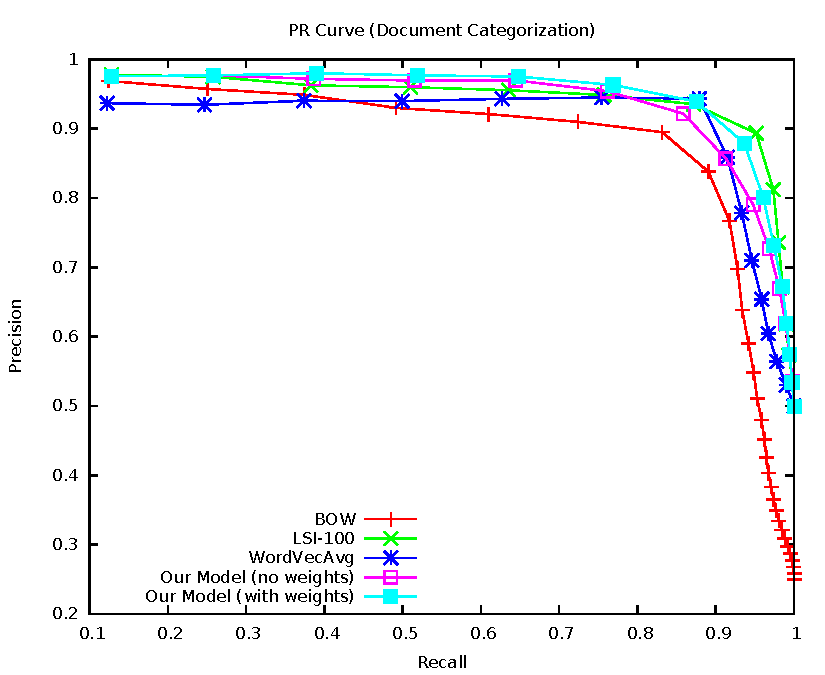
\includegraphics[width=0.7\columnwidth]{figs/pr/reuter-cs-scala.pdf}
        \vskip -4mm
    \caption{Precision/Recall for Document Categorization on Reuters-21578 (\emph{ModApte}) dataset} 
    \label{fig:pr:reuter:cs}
\end{figure}

%%%%%%%%%%%%%%%%%%%%%%%%%%%%%%%%%%%%%%%%%%%%%%  		Physics 		  %%%%%%%%%%%%%%%%%%%%%%%%%%%%%%%%%%%%%%%%%%%%%%%%%%%%%%%%%%%%%%%%%%%%%%%%%%%%%%%%%%%%%%%%%
\subsubsection{Physics - Wikipedia}
Performance of our model on the development data for different hyper-parameters is given in Table~\ref{physics:hp:k}, ~\ref{physics:hp:epoch}, ~\ref{physics:hp:c} and ~\ref{physics:hp:n}. We find that our model gives the best performance for $k=100$ (Table~\ref{physics:hp:k}) when trained for $150$ epochs (Table~\ref{physics:hp:epoch}). Table~\ref{physics:hp:c} shows that larger context window ($c = 3$) and default number of negative samples ($n = 10$) per positive sample gives the best performance. 

\begin{table}[h!]
\tabcolsep=0.1cm
\footnotesize
\begin{center}
\begin{tabular}{l@{\hskip5mm} c c@{\hskip4mm} c@{\hskip5mm} c c@{\hskip4mm} c@{\hskip5mm} c c@{\hskip4mm} c}
\toprule
& \multicolumn{9}{c}{\textbf{Hyper-parameters} : {$epochs = 50$, $c = 2$, $n = 10$}}         \\
\cmidrule(lr){2-10}
\textbf{Tuning}
& \multicolumn{3}{c}{{$k = 50$}}         
& \multicolumn{3}{c}{{$k = 100$}}        
& \multicolumn{3}{c}{{$k = 150$}}        	\\
\cmidrule(lr){2-4}
\cmidrule(lr){5-7}
\cmidrule(lr){8-10}
%\cmidrule(lr){2-10}
\multirow{2}{*}{\textbf{Physics} (Development)}
& {P} & {R} & \textbf{F1} 
& {P} & {R} & \textbf{F1} 
& {P} & {R} & \textbf{F1} \\
\cmidrule(lr){2-4}
\cmidrule(lr){5-7}
\cmidrule(lr){8-10}
& 84.4   & 72.1  & 77.8
& 89.1   & 71.2  & \highest{79.2}
& 89.1   & 69.7  & 78.2 \\
\bottomrule         
\end{tabular}
%\vskip -4mm
\caption{\label{physics:hp:k} Model performance on Physics(Wikipedia) development data for different embedding dimensionality}
\end{center}
\end{table}

\begin{table}[h!]
\tabcolsep=0.1cm
\footnotesize
\begin{center}
\begin{tabular}{l c c c c c c c c c c c c c c c}
\toprule
& \multicolumn{15}{c}{\textbf{Hyper-parameters} : {$k = 100$, $c = 2$, $n = 10$}}         \\
\cmidrule(lr){2-16}
\textbf{Tuning}
& \multicolumn{3}{c}{{$epochs = 20$}}         
& \multicolumn{3}{c}{{$epochs = 50$}}         
& \multicolumn{3}{c}{{$epochs = 100$}}         
& \multicolumn{3}{c}{{$epochs = 150$}}         
& \multicolumn{3}{c}{{$epochs = 200$}}	\\
\cmidrule(lr){2-4}
\cmidrule(lr){5-7}
\cmidrule(lr){8-10}
\cmidrule(lr){11-13}
\cmidrule(lr){14-16}
\multirow{2}{*}{\textbf{Physics} (Development)}
& {P} & {R} & \textbf{F1} 
& {P} & {R} & \textbf{F1} 
& {P} & {R} & \textbf{F1} 
& {P} & {R} & \textbf{F1} 
& {P} & {R} & \textbf{F1} \\
\cmidrule(lr){2-4}
\cmidrule(lr){5-7}
\cmidrule(lr){8-10}
\cmidrule(lr){11-13}
\cmidrule(lr){14-16}
& 85.5   & 70.6  & 77.3
& 89.1   & 71.2  & 79.2
& 86.9   & 73.8  & 79.9
& 87.4   & 73.6  & \highest{79.9}
& 86.9   & 73.3  & 79.5 \\
\bottomrule         
\end{tabular}
\caption{\label{physics:hp:epoch} Model performance on Physics(Wikipedia) development data for different number of epochs}
%\vskip -4mm
\end{center}
\end{table}

\begin{table}[h!]
\tabcolsep=0.1cm
\footnotesize
\begin{center}
\begin{tabular}{l@{\hskip5mm} c c@{\hskip4mm} c@{\hskip5mm} c c@{\hskip4mm} c@{\hskip5mm} c c@{\hskip4mm} c}
\toprule
& \multicolumn{9}{c}{\textbf{Hyper-parameters} : {$k = 100$, $epochs = 150$, $n = 10$}}         \\
\cmidrule(lr){2-10}
\textbf{Tuning}
& \multicolumn{3}{c}{{$c = 2$}}         
& \multicolumn{3}{c}{{$c = 3$}}        
& \multicolumn{3}{c}{{$c = 4$}}        	\\
\cmidrule(lr){2-4}
\cmidrule(lr){5-7}
\cmidrule(lr){8-10}
%\cmidrule(lr){2-10}
\multirow{2}{*}{\textbf{Physics} (Development)}
& {P} & {R} & \textbf{F1} 
& {P} & {R} & \textbf{F1} 
& {P} & {R} & \textbf{F1} \\
\cmidrule(lr){2-4}
\cmidrule(lr){5-7}
\cmidrule(lr){8-10}
& 87.4   & 73.6  & 79.9
& 86.5   & 74.4  & \highest{80.0}
& 87.0   & 73.1  & 79.5 \\
\bottomrule         
\end{tabular}
%\vskip -4mm
\caption{\label{physics:hp:c} Model performance on Physics(Wikipedia) development data for different window sizes}
\end{center}
\end{table}

\begin{table}[h!]
\tabcolsep=0.1cm
\footnotesize
\begin{center}
\begin{tabular}{l@{\hskip5mm} c c@{\hskip4mm} c@{\hskip5mm} c c@{\hskip4mm} c@{\hskip5mm} c c@{\hskip4mm} c}
\toprule
& \multicolumn{9}{c}{\textbf{Hyper-parameters} : {$k = 100$, $epochs = 150$, $c = 3$}}         \\
\cmidrule(lr){2-10}
\textbf{Tuning}
& \multicolumn{3}{c}{{$n = 5$}}         
& \multicolumn{3}{c}{{$n = 10$}}        
& \multicolumn{3}{c}{{$n = 15$}}        	\\
\cmidrule(lr){2-4}
\cmidrule(lr){5-7}
\cmidrule(lr){8-10}
%\cmidrule(lr){2-10}
\multirow{2}{*}{\textbf{Physics} (Development)}
& {P} & {R} & \textbf{F1} 
& {P} & {R} & \textbf{F1} 
& {P} & {R} & \textbf{F1} \\
\cmidrule(lr){2-4}
\cmidrule(lr){5-7}
\cmidrule(lr){8-10}
& 85.5   & 74.3  & 79.5
& 86.5   & 74.4  & \highest{80.0}
& 87.8   & 73.3  & 79.9 \\
\bottomrule         
\end{tabular}
%\vskip -4mm
\caption{\label{physics:hp:n} Model performance on Physics(Wikipedia) development data for different number of negative samples}
\end{center}
\end{table}

Table~\ref{physics:cs} shows that our model outperforms other baseline models with a huge margin. 
Our model achieves a F1 score of $79.7\%$ while the second best model, \textbf{BOW} trails ours by $2.31\%$.
As observed in the evaluation of Reuters-21578, syntactic features are necessary to learn high quality document representations. This is shown by the fact that when we simply sum the word vectors to represent the context, our model only achieves an accuracy of $73.8\%$ in terms of the F1 score.
Fig.~\ref{fig:pr:physics:cs} also shows that our model performs the best while \textbf{BOW} model is the second best performing model.

\begin{table}[h!]
\tabcolsep=0.1cm
\footnotesize
\begin{center}
\begin{tabular}{l@{\hskip5mm} c c@{\hskip4mm} c}
\toprule
% & \multicolumn{3}{c}{Reuters-21578}         \\
% \cmidrule(lr){2-4}
\textbf{Physics (Wikipedia)} & {P} & {R} & \textbf{F1} \\
\midrule
\textbf{BOW}
& 87.8   & 70.1  & 77.9 \\
\textbf{LSI-100}
& 83.4   & 69.5  & 75.8 \\
\textbf{WordVecAvg}
& 91.0   & 59.1  & 71.7 \\ \addlinespace[1mm]

\textbf{Our Model}
& \multirow{2}{*}{86.1}   & \multirow{2}{*}{64.6}  & \multirow{2}{*}{73.8} \\
(no weights) & & & \\ \addlinespace[1mm]
\textbf{Our Model}
& \multirow{2}{*}{88.6}   & \multirow{2}{*}{72.4}  & \multirow{2}{*}{\highest{79.7}} \\
(with weights) & & & \\
\bottomrule         
\end{tabular}
%\vskip -4mm
\caption{\label{physics:cs} Precision/Recall/F1 for Document Categorization on Physics(Wikipedia) dataset}
\end{center}
\end{table}

\begin{figure}[tb]
\centering
        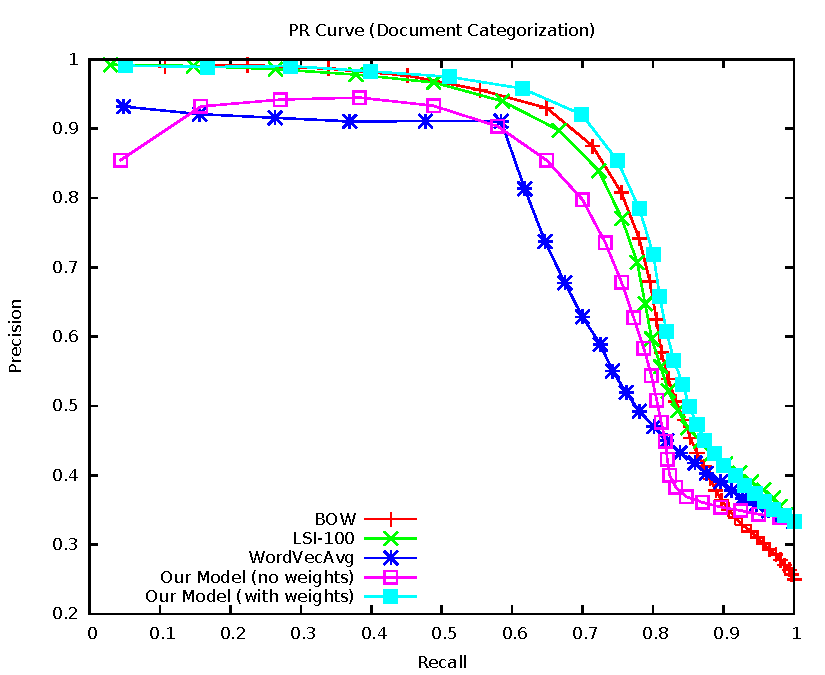
\includegraphics[width=0.7\columnwidth]{figs/pr/physics-cs-scala.pdf}
        \vskip -4mm
    \caption{ Precision/Recall for Document Categorization on Physics(Wikipedia) dataset}
    \label{fig:pr:physics:cs} 
\end{figure}

%%%%%%%%%%%%%%%%%%%%%%%%%%%%%%%%%%%%%%%%%%%%%%  		Biology 		  %%%%%%%%%%%%%%%%%%%%%%%%%%%%%%%%%%%%%%%%%%%%%%%%%%%%%%%%%%%%%%%%%%%%%%%%%%%%%%%%%%%%%%%%%
\subsubsection{Biology - Wikipedia}
The performance of our model on the development data for different values of hyper-parameters is shown in Table~\ref{biology:hp:k}, ~\ref{biology:hp:epoch}, ~\ref{biology:hp:c} and ~\ref{biology:hp:n}. Table~\ref{biology:hp:k} shows that default embedding size of $k = 100$ performs best and relatively low training epochs ($epochs = 50$) gives the best results (Table~\ref{biology:hp:epoch}). Larger context window ($c = 3$) (Table~\ref{biology:hp:c}) and default number of negative samples ($n = 10$) per positive sample (Table~\ref{biology:hp:n}) gives the best model performance. 

\begin{table}[h!]
\tabcolsep=0.1cm
\footnotesize
\begin{center}
\begin{tabular}{l@{\hskip5mm} c c@{\hskip4mm} c@{\hskip5mm} c c@{\hskip4mm} c@{\hskip5mm} c c@{\hskip4mm} c}
\toprule
& \multicolumn{9}{c}{\textbf{Hyper-parameters} : {$epochs = 50$, $c = 2$, $n = 10$}}         \\
\cmidrule(lr){2-10}
\textbf{Tuning}
& \multicolumn{3}{c}{{$k = 50$}}         
& \multicolumn{3}{c}{{$k = 100$}}        
& \multicolumn{3}{c}{{$k = 150$}}        	\\
\cmidrule(lr){2-4}
\cmidrule(lr){5-7}
\cmidrule(lr){8-10}
%\cmidrule(lr){2-10}
\multirow{2}{*}{\textbf{Biology} (Development)}
& {P} & {R} & \textbf{F1} 
& {P} & {R} & \textbf{F1} 
& {P} & {R} & \textbf{F1} \\
\cmidrule(lr){2-4}
\cmidrule(lr){5-7}
\cmidrule(lr){8-10}
& 83.9   & 60.0  & 70.0
& 82.4   & 61.2  & \highest{70.2}
& 83.7   & 60.2  & 70.0 \\
\bottomrule         
\end{tabular}
%\vskip -4mm
\caption{\label{biology:hp:k} Model performance on Biology(Wikipedia) development data for different embedding dimensionality}
\end{center}
\end{table}

\begin{table}[tb]
\tabcolsep=0.1cm
\footnotesize
\begin{center}
\begin{tabular}{l c c c c c c c c c c c c c c c}
\toprule
& \multicolumn{15}{c}{\textbf{Hyper-parameters} : {$k = 100$, $c = 2$, $n = 10$}}         \\
\cmidrule(lr){2-16}
\textbf{Tuning}
& \multicolumn{3}{c}{{$epochs = 20$}}         
& \multicolumn{3}{c}{{$epochs = 50$}}         
& \multicolumn{3}{c}{{$epochs = 100$}}         
& \multicolumn{3}{c}{{$epochs = 150$}}         
& \multicolumn{3}{c}{{$epochs = 200$}}	\\
\cmidrule(lr){2-4}
\cmidrule(lr){5-7}
\cmidrule(lr){8-10}
\cmidrule(lr){11-13}
\cmidrule(lr){14-16}
\multirow{2}{*}{\textbf{Biology} (Development)}
& {P} & {R} & \textbf{F1} 
& {P} & {R} & \textbf{F1} 
& {P} & {R} & \textbf{F1} 
& {P} & {R} & \textbf{F1} 
& {P} & {R} & \textbf{F1} \\
\cmidrule(lr){2-4}
\cmidrule(lr){5-7}
\cmidrule(lr){8-10}
\cmidrule(lr){11-13}
\cmidrule(lr){14-16}
& 75.3   & 59.8  & 66.7
& 82.4   & 61.2  & \highest{70.2}
& 82.9   & 60.2  & 69.7
& 85.6   & 58.6  & 69.6
& 85.3   & 58.0  & 69.0 \\
\bottomrule         
\end{tabular}
\caption{\label{biology:hp:epoch} Model performance on Biology(Wikipedia) development data for different number of epochs}
%\vskip -4mm
\end{center}
\end{table}

\begin{table}[h!]
\tabcolsep=0.1cm
\footnotesize
\begin{center}
\begin{tabular}{l@{\hskip5mm} c c@{\hskip4mm} c@{\hskip5mm} c c@{\hskip4mm} c@{\hskip5mm} c c@{\hskip4mm} c}
\toprule
& \multicolumn{9}{c}{\textbf{Hyper-parameters} : {$k = 100$, $epochs = 50$, $n = 10$}}         \\
\cmidrule(lr){2-10}
\textbf{Tuning}
& \multicolumn{3}{c}{{$c = 2$}}         
& \multicolumn{3}{c}{{$c = 3$}}        
& \multicolumn{3}{c}{{$c = 4$}}        	\\
\cmidrule(lr){2-4}
\cmidrule(lr){5-7}
\cmidrule(lr){8-10}
%\cmidrule(lr){2-10}
\multirow{2}{*}{\textbf{Biology} (Development)}
& {P} & {R} & \textbf{F1} 
& {P} & {R} & \textbf{F1} 
& {P} & {R} & \textbf{F1} \\
\cmidrule(lr){2-4}
\cmidrule(lr){5-7}
\cmidrule(lr){8-10}
& 82.4   & 61.2  & \highest{70.2}
& 80.8   & 62.0  & \highest{70.2}
& 81.3   & 61.4  & 70.0 \\
\bottomrule         
\end{tabular}
%\vskip -4mm
\caption{\label{biology:hp:c}Model performance on Biology(Wikipedia) development data for different window sizes}
\end{center}
\end{table}

\begin{table}[h!]
\tabcolsep=0.1cm
\footnotesize
\begin{center}
\begin{tabular}{l@{\hskip5mm} c c@{\hskip4mm} c@{\hskip5mm} c c@{\hskip4mm} c@{\hskip5mm} c c@{\hskip4mm} c}
\toprule
& \multicolumn{9}{c}{\textbf{Hyper-parameters} : {$k = 100$, $epochs = 50$, $c = 3$}}         \\
\cmidrule(lr){2-10}
\textbf{Tuning}
& \multicolumn{3}{c}{{$n = 5$}}         
& \multicolumn{3}{c}{{$n = 10$}}        
& \multicolumn{3}{c}{{$n = 15$}}        	\\
\cmidrule(lr){2-4}
\cmidrule(lr){5-7}
\cmidrule(lr){8-10}
%\cmidrule(lr){2-10}
\multirow{2}{*}{\textbf{Biology} (Development)}
& {P} & {R} & \textbf{F1} 
& {P} & {R} & \textbf{F1} 
& {P} & {R} & \textbf{F1} \\
\cmidrule(lr){2-4}
\cmidrule(lr){5-7}
\cmidrule(lr){8-10}
& 81.8   & 61.0  & 69.9
& 80.8   & 62.0  & \highest{70.2}
& 81.2   & 60.8  & 69.6 \\
\bottomrule         
\end{tabular}
%\vskip -4mm
\caption{\label{biology:hp:n}Model performance on Biology(Wikipedia) development data for different number of negative samples}
\end{center}
\end{table}

Table~\ref{biology:cs} shows that the distributed representations learned by our model outperform some baseline representations but the bag-of-words representation works the best.
Our model achieves a F1 score of $67.8\%$ while the \textbf{BOW} improves our model by $1.7\%$.
We also find that document representations learned by averaging word vectors performs the worst. The model accuracy suffers by $4.95\%$ when context word weighting is ignored during training.
Fig.~\ref{fig:pr:biology:cs} shows the precision/recall curves for our model and other baseline methods. It also shows that the \textbf{BOW} representations perform the closest to representations learned using our model.

\begin{table}[h!]
\tabcolsep=0.1cm
\footnotesize
\begin{center}
\begin{tabular}{l@{\hskip5mm} c c@{\hskip4mm} c}
\toprule
% & \multicolumn{3}{c}{Reuters-21578}         \\
% \cmidrule(lr){2-4}
\textbf{Biology (Wikipedia)} & {P} & {R} & \textbf{F1} \\
\midrule
\textbf{BOW}
& 90.3   & 59.5  & \highest{69.0} \\
\textbf{LSI-100}
& 82.1   & 51.6  & 63.4 \\
\textbf{WordVecAvg}
& 79.4   & 50.4  & 61.6 \\ \addlinespace[1mm]

\textbf{Our Model}
& \multirow{2}{*}{80.3}   & \multirow{2}{*}{53.8}  & \multirow{2}{*}{64.4} \\
(no weights) & & & \\ \addlinespace[1mm]
\textbf{Our Model}
79.7  R :  59.0  F1 :  67.8
& \multirow{2}{*}{79.7}   & \multirow{2}{*}{59.0}  & \multirow{2}{*}{67.8} \\
(with weights) & & & \\
\bottomrule         
\end{tabular}
%\vskip -4mm
\caption{\label{biology:cs} Precision/Recall/F1 for Document Categorization on Biology(Wikipedia) dataset}
\end{center}
\end{table}

\begin{figure}[tb]
\centering
        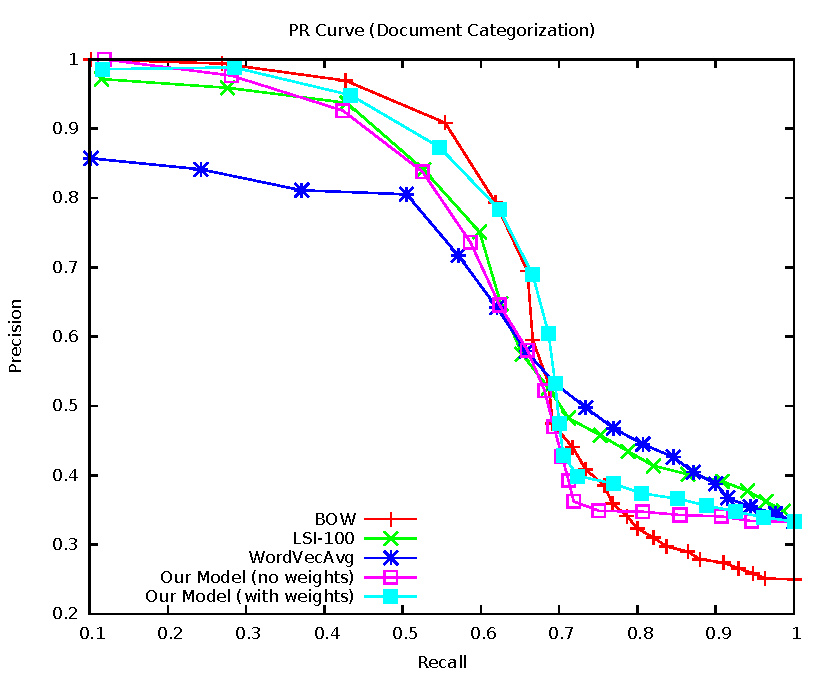
\includegraphics[width=0.7\columnwidth]{figs/pr/biology-cs-scala.pdf}
        \vskip -4mm
    \caption{ Precision/Recall for Document Categorization on Biology(Wikipedia) dataset}
    \label{fig:pr:biology:cs} 
\end{figure}

%%%%%%%%%%%%%%%%%%%%%%%%%%%%%%%%%%%%%%%%%%%%%%  		Mathematics 		  %%%%%%%%%%%%%%%%%%%%%%%%%%%%%%%%%%%%%%%%%%%%%%%%%%%%%%%%%%%%%%%%%%%%%%%%%%%%%%%%%%%%%%%%%
\subsubsection{Mathematics - Wikipedia}
Table~\ref{mathematics:hp:k}, ~\ref{mathematics:hp:epoch}, ~\ref{mathematics:hp:c} and ~\ref{mathematics:hp:n} show that low embedding size of $k = 50$ and moderate training epochs ($epochs = 100$) give the best model performance. We also find that relatively larger context window ($c = 3$) and number of negative samples ($n = 15$) per positive sample are required for optimal model performance.

\begin{table}[h!]
\tabcolsep=0.1cm
\footnotesize
\begin{center}
\begin{tabular}{l@{\hskip5mm} c c@{\hskip4mm} c@{\hskip5mm} c c@{\hskip4mm} c@{\hskip5mm} c c@{\hskip4mm} c}
\toprule
& \multicolumn{9}{c}{\textbf{Hyper-parameters} : {$epochs = 50$, $c = 2$, $n = 10$}}         \\
\cmidrule(lr){2-10}
\textbf{Tuning}
& \multicolumn{3}{c}{{$k = 50$}}         
& \multicolumn{3}{c}{{$k = 100$}}        
& \multicolumn{3}{c}{{$k = 150$}}        	\\
\cmidrule(lr){2-4}
\cmidrule(lr){5-7}
\cmidrule(lr){8-10}
%\cmidrule(lr){2-10}
\multirow{2}{*}{\textbf{Mathematics} (Development)}
& {P} & {R} & \textbf{F1} 
& {P} & {R} & \textbf{F1} 
& {P} & {R} & \textbf{F1} \\
\cmidrule(lr){2-4}
\cmidrule(lr){5-7}
\cmidrule(lr){8-10}
& 83.2   & 57.0  & \highest{67.7}
& 82.3   & 56.0  & 66.7
& 86.1   & 55.5  & 67.5 \\
\bottomrule         
\end{tabular}
%\vskip -4mm
\caption{\label{mathematics:hp:k} Model performance on Mathematics(Wikipedia) development data for different embedding dimensionality}
\end{center}
\end{table}

\begin{table}[h!]
\tabcolsep=0.1cm
\footnotesize
\begin{center}
\begin{tabular}{l c c c c c c c c c c c c c c c}
\toprule
& \multicolumn{15}{c}{\textbf{Hyper-parameters} : {$k = 50$, $c = 2$, $n = 10$}}         \\
\cmidrule(lr){2-16}
\textbf{Tuning}
& \multicolumn{3}{c}{{$epochs = 20$}}         
& \multicolumn{3}{c}{{$epochs = 50$}}         
& \multicolumn{3}{c}{{$epochs = 100$}}         
& \multicolumn{3}{c}{{$epochs = 150$}}         
& \multicolumn{3}{c}{{$epochs = 200$}}	\\
\cmidrule(lr){2-4}
\cmidrule(lr){5-7}
\cmidrule(lr){8-10}
\cmidrule(lr){11-13}
\cmidrule(lr){14-16}
\multirow{2}{*}{\textbf{Mathematics} (Development)}
& {P} & {R} & \textbf{F1} 
& {P} & {R} & \textbf{F1} 
& {P} & {R} & \textbf{F1} 
& {P} & {R} & \textbf{F1} 
& {P} & {R} & \textbf{F1} \\
\cmidrule(lr){2-4}
\cmidrule(lr){5-7}
\cmidrule(lr){8-10}
\cmidrule(lr){11-13}
\cmidrule(lr){14-16}
& 81.2   & 55.2  & 65.8
& 83.2   & 57.0  & 67.7
& 87.0   & 56.3  & \highest{68.3}
& 86.7   & 55.2  & 67.5
& 82.2   & 57.8  & 67.9 \\
\bottomrule         
\end{tabular}
\caption{\label{mathematics:hp:epoch} Model performance on Mathematics(Wikipedia) development data for different number of epochs}
%\vskip -4mm
\end{center}
\end{table}

\begin{table}[h!]
\tabcolsep=0.1cm
\footnotesize
\begin{center}
\begin{tabular}{l@{\hskip5mm} c c@{\hskip4mm} c@{\hskip5mm} c c@{\hskip4mm} c@{\hskip5mm} c c@{\hskip4mm} c}
\toprule
& \multicolumn{9}{c}{\textbf{Hyper-parameters} : {$k = 50$, $epochs = 100$, $n = 10$}}         \\
\cmidrule(lr){2-10}
\textbf{Tuning}
& \multicolumn{3}{c}{{$c = 2$}}         
& \multicolumn{3}{c}{{$c = 3$}}        
& \multicolumn{3}{c}{{$c = 4$}}        	\\
\cmidrule(lr){2-4}
\cmidrule(lr){5-7}
\cmidrule(lr){8-10}
%\cmidrule(lr){2-10}
\multirow{2}{*}{\textbf{Mathematics} (Development)}
& {P} & {R} & \textbf{F1} 
& {P} & {R} & \textbf{F1} 
& {P} & {R} & \textbf{F1} \\
\cmidrule(lr){2-4}
\cmidrule(lr){5-7}
\cmidrule(lr){8-10}
& 87.0   & 56.3  & \highest{68.3}
& 91.0   & 54.5  & 68.2
& 88.1   & 55.0  & 67.7 \\
\bottomrule         
\end{tabular}
%\vskip -4mm
\caption{\label{mathematics:hp:c} Model performance on Mathematics(Wikipedia) development data for different window sizes}
\end{center}
\end{table}

\begin{table}[h!]
\tabcolsep=0.1cm
\footnotesize
\begin{center}
\begin{tabular}{l@{\hskip5mm} c c@{\hskip4mm} c@{\hskip5mm} c c@{\hskip4mm} c@{\hskip5mm} c c@{\hskip4mm} c}
\toprule
& \multicolumn{9}{c}{\textbf{Hyper-parameters} : {$k = 50$, $epochs = 100$, $c = 2$}}         \\
\cmidrule(lr){2-10}
\textbf{Tuning}
& \multicolumn{3}{c}{{$n = 5$}}         
& \multicolumn{3}{c}{{$n = 10$}}        
& \multicolumn{3}{c}{{$n = 15$}}        	\\
\cmidrule(lr){2-4}
\cmidrule(lr){5-7}
\cmidrule(lr){8-10}
%\cmidrule(lr){2-10}
\multirow{2}{*}{\textbf{Mathematics} (Development)}
& {P} & {R} & \textbf{F1} 
& {P} & {R} & \textbf{F1} 
& {P} & {R} & \textbf{F1} \\
\cmidrule(lr){2-4}
\cmidrule(lr){5-7}
\cmidrule(lr){8-10}
& 86.1   & 57.0  & 68.6
& 87.0   & 56.3  & 68.3
& 90.0   & 55.5  & \highest{68.7} \\
\bottomrule         
\end{tabular}
%\vskip -4mm
\caption{\label{mathematics:hp:n} Model performance on Mathematics(Wikipedia) development data for different number of negative samples}
\end{center}
\end{table}

Table~\ref{mathematics:cs} shows that the distributed representations learned by our model outperform other baseline representations.
Our model achieves a F1 score of $68.2\%$ while the second best model, \textbf{BOW} trails ours by $4.41\%$.
Word vectors averaged by tf-idf weighing scheme to represent document in the Mathematics (Wikipedia) dataset give the worst accuracy with an F1 score of $55.7\%$.
We again find that modeling syntactic qualities of the language is important as weighting word vectors to represent the context gives the best performance.
Fig.~\ref{fig:pr:mathematics:cs} shows the precision/recall curves for our model and other baseline methods. 

\begin{table}[h!]
\tabcolsep=0.1cm
\footnotesize
\begin{center}
\begin{tabular}{l@{\hskip5mm} c c@{\hskip4mm} c}
\toprule
% & \multicolumn{3}{c}{Reuters-21578}         \\
% \cmidrule(lr){2-4}
\textbf{Mathematics (Wikipedia)} & {P} & {R} & \textbf{F1} \\
\midrule
\textbf{BOW}
& 65.6   & 65.1  & 65.3 \\
\textbf{LSI-100}
& 89.7   & 50.3  & 64.4 \\
\textbf{WordVecAvg}
& 90.5   & 40.3  & 55.7 \\ \addlinespace[1mm]

\textbf{Our Model}
& \multirow{2}{*}{78.4}   & \multirow{2}{*}{57.4}  & \multirow{2}{*}{66.3} \\
(no weights) & & & \\ \addlinespace[1mm]
\textbf{Our Model}
& \multirow{2}{*}{85.3}   & \multirow{2}{*}{56.8}  & \multirow{2}{*}{\highest{68.2}} \\
(with weights) & & & \\
\bottomrule         
\end{tabular}
%\vskip -4mm
\caption{\label{mathematics:cs} Precision/Recall/F1 for Document Categorization on Mathematics(Wikipedia) dataset}
\end{center}
\end{table}

\begin{figure}[tb]
\centering
        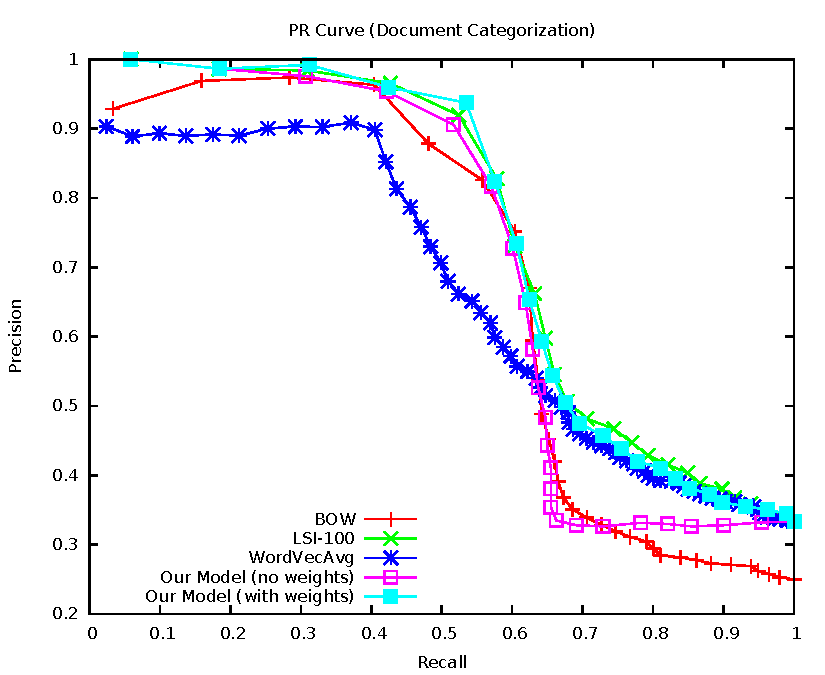
\includegraphics[width=0.7\columnwidth]{figs/pr/mathematics-cs-scala.pdf}
        \vskip -4mm
    \caption{ Precision/Recall for Document Categorization on Mathematics(Wikipedia) dataset}
    \label{fig:pr:mathematics:cs} 
\end{figure}

%%%%%%%%%%%%%%%%%%%%%%%%%%%%%%%%%%%%%%%%%%%%%%  		Sports 		  %%%%%%%%%%%%%%%%%%%%%%%%%%%%%%%%%%%%%%%%%%%%%%%%%%%%%%%%%%%%%%%%%%%%%%%%%%%%%%%%%%%%%%%%%
\subsubsection{Sports - Wikipedia}
The performance of our model on the development data for different values of different hyper-parameters is shown in Table~\ref{sports:hp:k}, ~\ref{sports:hp:epoch}, ~\ref{sports:hp:c} and ~\ref{sports:hp:n}. Table~\ref{sports:hp:k} shows that low vector size of $k = 50$ and Table~\ref{sports:hp:epoch} shows moderate training epochs ($epochs = 100$) gives the best model performance. 
Table~\ref{sports:hp:c} shows that context window size of $c = 3$ and relatively larger number of negative samples ($n = 15$) per positive sample achieves the best performance.

\begin{table}[h!]
\tabcolsep=0.1cm
\footnotesize
\begin{center}
\begin{tabular}{l@{\hskip5mm} c c@{\hskip4mm} c@{\hskip5mm} c c@{\hskip4mm} c@{\hskip5mm} c c@{\hskip4mm} c}
\toprule
& \multicolumn{9}{c}{\textbf{Hyper-parameters} : {$epochs = 50$, $c = 2$, $n = 10$}}         \\
\cmidrule(lr){2-10}
\textbf{Tuning}
& \multicolumn{3}{c}{{$k = 50$}}         
& \multicolumn{3}{c}{{$k = 100$}}        
& \multicolumn{3}{c}{{$k = 150$}}        	\\
\cmidrule(lr){2-4}
\cmidrule(lr){5-7}
\cmidrule(lr){8-10}
%\cmidrule(lr){2-10}
\multirow{2}{*}{\textbf{Sports} (Development)}
& {P} & {R} & \textbf{F1} 
& {P} & {R} & \textbf{F1} 
& {P} & {R} & \textbf{F1} \\
\cmidrule(lr){2-4}
\cmidrule(lr){5-7}
\cmidrule(lr){8-10}
& 82.2   & 45.7  & \highest{58.8}
& 81.2   & 45.9  & 58.6
& 80.9   & 45.7  & 58.4 \\
\bottomrule         
\end{tabular}
%\vskip -4mm
\caption{\label{sports:hp:k} Model performance on Sports(Wikipedia) development data for different embedding dimensionality}
\end{center}
\end{table}

\begin{table}[tb]
\tabcolsep=0.1cm
\footnotesize
\begin{center}
\begin{tabular}{l c c c c c c c c c c c c c c c}
\toprule
& \multicolumn{15}{c}{\textbf{Hyper-parameters} : {$k = 50$, $c = 2$, $n = 10$}}         \\
\cmidrule(lr){2-16}
\textbf{Tuning}
& \multicolumn{3}{c}{{$epochs = 20$}}         
& \multicolumn{3}{c}{{$epochs = 50$}}         
& \multicolumn{3}{c}{{$epochs = 100$}}         
& \multicolumn{3}{c}{{$epochs = 150$}}         
& \multicolumn{3}{c}{{$epochs = 200$}}	\\
\cmidrule(lr){2-4}
\cmidrule(lr){5-7}
\cmidrule(lr){8-10}
\cmidrule(lr){11-13}
\cmidrule(lr){14-16}
\multirow{2}{*}{\textbf{Sports} (Development)}
& {P} & {R} & \textbf{F1} 
& {P} & {R} & \textbf{F1} 
& {P} & {R} & \textbf{F1} 
& {P} & {R} & \textbf{F1} 
& {P} & {R} & \textbf{F1} \\
\cmidrule(lr){2-4}
\cmidrule(lr){5-7}
\cmidrule(lr){8-10}
\cmidrule(lr){11-13}
\cmidrule(lr){14-16}
& 73.9   & 45.9  & 56.6
& 82.2   & 45.7  & 58.8
& 83.9   & 47.6  & \highest{60.7}
& 83.7   & 46.8  & 60.0
& 67.1   & 50.2  & 57.4 \\
\bottomrule         
\end{tabular}
\caption{\label{sports:hp:epoch}  Model performance on Sports(Wikipedia) development data for different number of epochs}
%\vskip -4mm
\end{center}
\end{table}

\begin{table}[h!]
\tabcolsep=0.1cm
\footnotesize
\begin{center}
\begin{tabular}{l@{\hskip5mm} c c@{\hskip4mm} c@{\hskip5mm} c c@{\hskip4mm} c@{\hskip5mm} c c@{\hskip4mm} c}
\toprule
& \multicolumn{9}{c}{\textbf{Hyper-parameters} : {$k = 50$, $epochs = 100$, $n = 10$}}         \\
\cmidrule(lr){2-10}
\textbf{Tuning}
& \multicolumn{3}{c}{{$c = 2$}}         
& \multicolumn{3}{c}{{$c = 3$}}        
& \multicolumn{3}{c}{{$c = 4$}}        	\\
\cmidrule(lr){2-4}
\cmidrule(lr){5-7}
\cmidrule(lr){8-10}
%\cmidrule(lr){2-10}
\multirow{2}{*}{\textbf{Sports} (Development)}
& {P} & {R} & \textbf{F1} 
& {P} & {R} & \textbf{F1} 
& {P} & {R} & \textbf{F1} \\
\cmidrule(lr){2-4}
\cmidrule(lr){5-7}
\cmidrule(lr){8-10}
& 83.9   & 47.6  & 60.7
& 84.5   & 47.8  & \highest{61.0}
& 86.0   & 47.0  & 60.8 \\
\bottomrule         
\end{tabular}
%\vskip -4mm
\caption{\label{sports:hp:c} Model performance on Sports(Wikipedia) development data for different window sizes}
\end{center}
\end{table}

\begin{table}[h!]
\tabcolsep=0.1cm
\footnotesize
\begin{center}
\begin{tabular}{l@{\hskip5mm} c c@{\hskip4mm} c@{\hskip5mm} c c@{\hskip4mm} c@{\hskip5mm} c c@{\hskip4mm} c}
\toprule
& \multicolumn{9}{c}{\textbf{Hyper-parameters} : {$k = 50$, $epochs = 100$, $c = 3$}}         \\
\cmidrule(lr){2-10}
\textbf{Tuning}
& \multicolumn{3}{c}{{$n = 5$}}         
& \multicolumn{3}{c}{{$n = 10$}}        
& \multicolumn{3}{c}{{$n = 15$}}        	\\
\cmidrule(lr){2-4}
\cmidrule(lr){5-7}
\cmidrule(lr){8-10}
%\cmidrule(lr){2-10}
\multirow{2}{*}{\textbf{Sports} (Development)}
& {P} & {R} & \textbf{F1} 
& {P} & {R} & \textbf{F1} 
& {P} & {R} & \textbf{F1} \\
\cmidrule(lr){2-4}
\cmidrule(lr){5-7}
\cmidrule(lr){8-10}
& 84.6   & 47.0  & 60.4
& 84.5   & 47.8  & \highest{61.0}
& 82.7   & 47.4  & 60.3 \\
\bottomrule         
\end{tabular}
%\vskip -4mm
\caption{\label{sports:hp:n} Model performance on Sports(Wikipedia) development data for different number of negative samples}
\end{center}
\end{table}

Table~\ref{sports:cs} shows that the distributed representations learned by our model outperform other baseline representations.
Our model achieves a F1 score of $57.3\%$ while again the \textbf{BOW} model is second best performing.
As found in previous evaluations, document representations using bag-of-words style word vector averaging perform the worst and modeling syntactic features is important for learning the best quality document representations.
Fig.~\ref{fig:pr:sports:cs} shows the precision/recall curves for our model and other baseline methods. 

\begin{table}[h!]
\tabcolsep=0.1cm
\footnotesize
\begin{center}
\begin{tabular}{l@{\hskip5mm} c c@{\hskip4mm} c}
\toprule
% & \multicolumn{3}{c}{Reuters-21578}         \\
% \cmidrule(lr){2-4}
\textbf{Sports (Wikipedia)} & {P} & {R} & \textbf{F1} \\
\midrule
\textbf{BOW}
& 91.7   & 41.3  & 56.9 \\
\textbf{LSI-100}
& 91.2   & 40.1  & 55.7 \\
\textbf{WordVecAvg}
& 81.8   & 37.5  & 51.4 \\ \addlinespace[1mm]

\textbf{Our Model}
& \multirow{2}{*}{80.5}   & \multirow{2}{*}{40.1}  & \multirow{2}{*}{53.6} \\
(no weights) & & & \\ \addlinespace[1mm]
\textbf{Our Model}
& \multirow{2}{*}{82.1}   & \multirow{2}{*}{44.0}  & \multirow{2}{*}{\highest{57.3}} \\
(with weights) & & & \\
\bottomrule         
\end{tabular}
%\vskip -4mm
\caption{\label{sports:cs} Precision/Recall/F1 for Document Categorization on Sports(Wikipedia) dataset}
\end{center}
\end{table}

\begin{figure}[tb]
\centering
        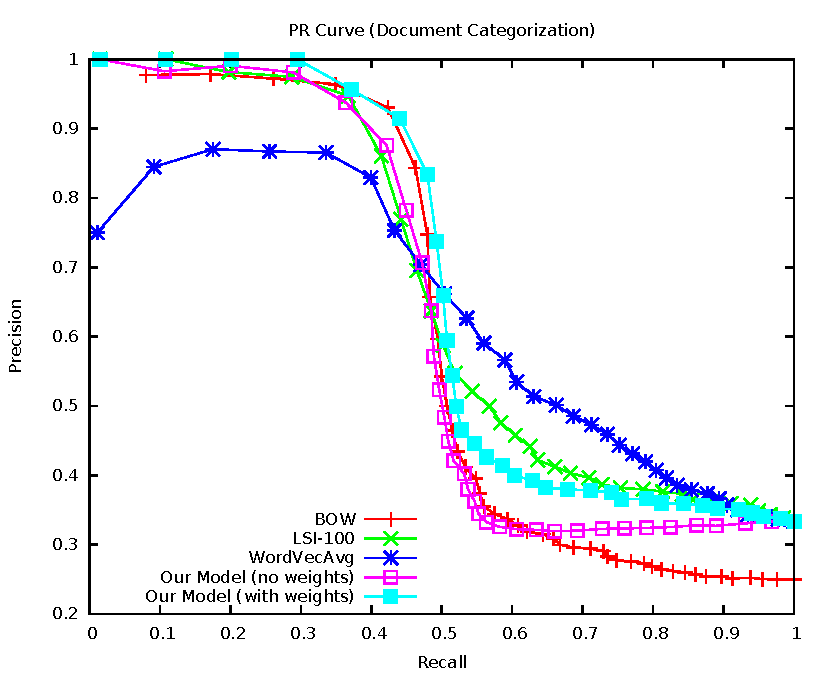
\includegraphics[width=0.7\columnwidth]{figs/pr/sports-cs-scala.pdf}
        \vskip -4mm
    \caption{Precision/Recall for Document Categorization on Sports(Wikipedia) dataset}
    \label{fig:pr:sports:cs} 
\end{figure}

%%%%%%%%%%%%%%%%%%%%%%%%%%%%%			IMPUTING MISSING CAEGORIES 				%%%%%%%%%%%%%%%%%%%%%%%%%%%%%%%%%%%%%%%%%%%%%%%%%%%%%%%%%%%%%%%%%%%%%%%%%%%%%%%%%%%%%%%%%%%%%%
\subsection{Imputing Missing Categories}
\label{sec:results:imputing}
Most of the real-life databases that contain categorization for documents contain incomplete information. In the case of huge number of categories and when document categorization is carried out by non-experts, as in Wikipedia, one can never be sure that all the relevant categories have been assigned to each document. In such large-scale databases where manual annotation and review is difficult, systems that can automatically impute missing categories for documents in the database are imperative.

In this section we evaluate our system's efficacy in imputing missing categories in the Wikipedia datasets.  
The task is similar to Relational Learning where the task is to complete the sparse relational matrix, $R$ between two types of entities. 
In our case, we estimate the probability of every unobserved document-category pair $(d_{i}, c_{k})$ to be true to complete the sparse document-category matrix in which only positive document-category pairs are observed.
For training and testing purposes, we first introduce corrupt document-category pairs as negative samples in the training data $\traindata$ in the following manner. For every positive $\{ d_{i}, c_{j}, 1\}$ observed in the training data, we introduce two negative samples $\{ d_{i}, c_{k}, 0\}$ where the negative sampled category $c'_{k}$ is chosen uniformly for the category set. This increases the tuples in the training data by three times. From the modified training data we randomly choose $80\%$ document-category pairs for training purposes and divide the rest equally for development and test purposes. The document representations are learned in the same manner as in the previous evaluation.

Table~\ref{wikipedia:ho} shows our model's efficacy in imputing missing categories in the different Wikipedia datasets. We also compute a combined F1 score for all the datasets in the micro-averaged fashion, i.e. by combining all the prediction for all the datasets and then computing the precision and the recall. 
As expected our model of learning distributed document representations outperforms all other baselines by a large margin. 
Our model achieves an overall F1 score of $74.3\%$ which improves upon the bag-of-words (\textbf{BOW}) model by $4.78\%$. 
Representing documents by averaging the word vectors using \emph{tf-idf} weighing scheme achieves a F1 score of $65.4\%$. 
The worst performing model, as expected is \textbf{PMF} which does not use any textual information about the documents.
As found in the previous section, in our model, simple summing of context word vectors to represent the context does not provide competitive results which corroborates the hypothesis that encoding syntactic information is necessary. 
%Figure~\ref{fig:pr:wiki:ho} shows the precision/recall curves for the different document representation models along with the performance of our models.

\begin{table}[h!]
\tabcolsep=1mm
\footnotesize
\begin{center}
%\begin{tabular}{l cc@{\hskip 2mm}c@{\hskip 2mm} cc@{\hskip 2mm}c@{\hskip 2mm} cc@{\hskip 2mm}c@{\hskip 2mm} cc@{\hskip 2mm}c@{\hskip 2mm} cc@{\hskip 2mm}c}
\begin{tabular}{l ccc@{\hskip 3mm} ccc@{\hskip 3mm} ccc@{\hskip 3mm} ccc@{\hskip 3mm} ccc}
\toprule
\multirow{2}{*}{} & 
\multicolumn{3}{c}{{Physics}}         & 
\multicolumn{3}{c}{{Biology}}        & \multicolumn{3}{c}{{Mathematics}}         & \multicolumn{3}{c}{{Sports}}        & %\multicolumn{3}{c}{\textbf{Restaurant}}       & 
\multicolumn{3}{c}{\textbf{Combined}}              
\\ 
\cmidrule(lr){2-4}
\cmidrule(lr){5-7}
\cmidrule(lr){8-10}
\cmidrule(lr){11-13}
\cmidrule(lr){14-16}
& 
{P} & {R} & \textbf{F1} & 
{P} & {R} & \textbf{F1} & 
{P} & {R} & \textbf{F1} & 
{P} & {R} & \textbf{F1} &
{P} & {R} & \textbf{F1} \\ 
\midrule
\textbf{PMF}
& 73.0   & 64.3  & 68.4
& 72.1   & 47.5  & 57.3
& 41.6   & 58.2  & 48.5
& 51.3   & 35.6  & 42.0
& 63.0   & 54.8  & 58.6 
\\
\textbf{LSI-100}
& 59.5   & 82.3  & 69.0
& 49.9   & 71.6  & 58.8
& 47.1   & 73.0  & 57.3
& 43.1   & 68.2  & 52.8
& 52.5   & 76.3  & 62.2
\\ 
\textbf{BOW}
& 76.1   & 79.4  & 77.7
& 69.7   & 67.7  & 68.7
& 70.9   & 63.5  & 67.0
& 64.8   & 49.3  & 56.0
& 72.5   & 69.4  & 70.9
\\
\textbf{WordVecAvg}
& 88.0   & 63.5  & 73.8
& 80.7   & 50.3  & 61.9
& 71.8   & 46.7  & 56.6
& 87.2   & 35.4  & 50.3
& 84.2   & 53.4  & 65.4
\\ \addlinespace[1mm]
\textbf{Our Model}
& \multirow{2}{*}{88.6}   & \multirow{2}{*}{69.1}  & \multirow{2}{*}{77.7}
& \multirow{2}{*}{80.5}   & \multirow{2}{*}{55.3}  & \multirow{2}{*}{65.6}
& \multirow{2}{*}{74.3}   & \multirow{2}{*}{53.1}  & \multirow{2}{*}{61.9}
& \multirow{2}{*}{84.7}   & \multirow{2}{*}{40.2}  & \multirow{2}{*}{54.5}
& \multirow{2}{*}{85.4}   & \multirow{2}{*}{58.5}  & \multirow{2}{*}{69.2}
\\ 
(without weights) & & & & & & & & & & & & & &  & \\
\addlinespace[1mm]
\textbf{Our Model}
& \multirow{2}{*}{89.9}   & \multirow{2}{*}{74.5}  & \multirow{2}{*}{\highest{81.5}}
& \multirow{2}{*}{84.9}   & \multirow{2}{*}{63.8} & \multirow{2}{*}{\highest{72.9}}
& \multirow{2}{*}{79.9}   & \multirow{2}{*}{60.7}  & \multirow{2}{*}{\highest{69.0}}
& \multirow{2}{*}{81.1}   & \multirow{2}{*}{45.6} & \multirow{2}{*}{\highest{58.4}}
& \multirow{2}{*}{86.3}   & \multirow{2}{*}{65.2}  & \multirow{2}{*}{\highest{74.3}}
\\ 
(with weights) & & & & & & & & & & & & & &  & \\
\bottomrule         
\end{tabular}
\end{center}
\caption{\label{wikipedia:ho} Precision/Recall/F1 for Imputing Missing Categories in the Wikipedia Datasets }
\end{table}
% \begin{figure}[tb]
% \centering
%         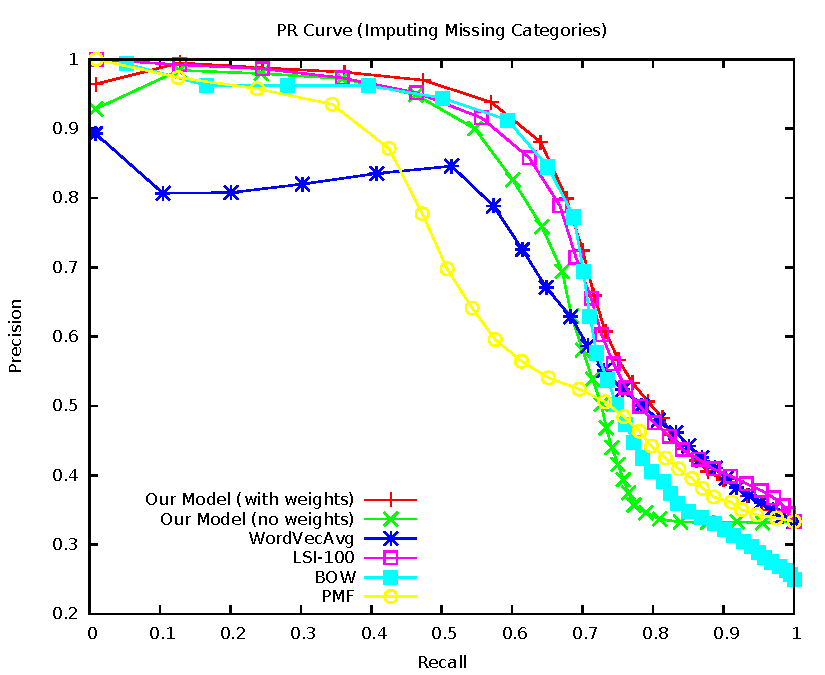
\includegraphics[width=0.8\columnwidth]{figs/pr/wiki-ho-scala.pdf}
%         \vskip -4mm
%     \caption{\footnotesize Precision/Recall for Imputing Missing Categories on the Wikipedia datasets}
%     \label{fig:pr:wiki:ho} 
% \end{figure}

\subsection{Estimating Similarity between Categories and Words}
One of the primary drawbacks faced by the bag-of-words representations is the lack of similarity measures due to the discrete nature of the representation vectors. 
Also, when documents are represented using bag-of-words vectors, there is no representation for the words in the vocabulary. 
As we show in our model, we embed words and documents in the same k-dimensional space such that semantically similar entities have similar vector representations. 

One of the biggest advantages of using the modified logistic regression algorithm is that we learn distributed category representations in the same $k$-dimensional space as the semantic space of words and documents. Such representations allow us to compute similarity between indirectly related entities such as words and categories. 
Estimating the similarity or distance between two entities is equivalent to taking the dot-product between their representation vectors.

In Table~\ref{catword:sim} we present a few random categories along with their nearest neighboring words as found using the representations learned using our model. 
We see that the representations learned using our model can successfully encode the semantic similarity between entities, categories and words in this case.
For example, we see that the words closest to the category \emph{Evolutionary Biology} are \emph{Darwin}, \emph{lineage}, \emph{phylogenetics}, closest to category \emph{Thermodynamics} are \emph{convection}, \emph{enthalpy}, \emph{calorimetric} and closest to category \emph{Theoretical Physicists} are world famous physicists such as \emph{Dipankar}, \emph{Uri}, \emph{Aneesur}.

\begin{table}[h!]
\tabcolsep=1mm
\footnotesize
\begin{center}
\begin{adjustwidth}{-1.5cm}{}
\begin{tabular}{l@{\hskip3mm} l}
\toprule
\multirow{2}{*}{\textbf{Category}} & \multirow{2}{*}{\textbf{Nearest Neighbors}} \\
 & \\
%\cmidrule{2-2}
\textbf{Evolutionary Biology}   & gene, phylogenetics, speciation, ancestor, Darwin, lineage, evolutionary, interbreeding \\
\textbf{Statistical Mechanics}  & ergodicity, Eigenstate, Universality, DMFT, Markovian, Parisi, Combinatorics \\
\textbf{Thermodynamics}         & Convection, ecosystem, Enthalpy, Joule, calorimetric, compressible, Thermodynamic \\
\textbf{Trade}                  & import, Pledges, Tariff, Trade, competitiveness, toll, billion, basket, Ditch, Worldwide \\
\textbf{Money-FX}               & Borrowing, franc, banker, Currency, banks, nervous, sideways, Markets, FORWARD \\
\textbf{Virology}               & nucleoside, ribozyme, adenoviruses, Virology, retroviruses, poliovirus, Viroid \\
\textbf{Neurobiology}           & purinergic, cyclase, vertebral, Ehrlich, nexus, steroid, lean, gendered, reticular \\
\textbf{Physical Exercise}      & Fitness, aerobics, metabolic, workout, Exercise, Stretching, pelvic, Physiology, fibers \\
\textbf{Algebra}                & subalgebra, Algebras, nilpotent, adjoints, octonions, bicommutant, diagonalizable \\
\textbf{Theoretical Physicists} & Dipankar, DSc, Hubert, Aneesur, Uri, Ignaz, Chia, Stig, Diderot, Dannie \\
\textbf{Mathematical Physics}   & covectors, pseudotensor, spacelike, dyadic, Curl, torque, contractions, wavefunctions \\
\textbf{Sports Venues}          & stadion, decoration, tracks, seating, buildings, parcourse, architectural, arenas, circular \\
\textbf{Indian Mathematics}     & utkrama, ecliptic, Siddhanta, Hellenistic, Brahmi, sexagesimal, scribe, Islamic, Sanskrit \\
\bottomrule         
\end{tabular}
 \end{adjustwidth}
\end{center}
\caption{\label{catword:sim} Estimating Similarity between Categories and Words}
\end{table}